\section{Suitability of Different Qubit Types for Quantum Error Correction}
\label{section: qec}
In the following section, different qubit types will be compared for their potential to be used in FTQC. For usable QEC, DiVincenzo proposed five basic requirements of an ideal qubit: sufficiently long T1/T2 times (i), fast and reliable gate operations (ii), initialization (iii) and readout (iv), and scalability for large-scale architectures (v) \cite{DIVINCENZO1998419}.  Additionally, the implementation of QEC is partly determined by noise type, working temperature and connectivity. Table \ref{tab:qubit_comparison} contains a comprehensive overview of superconducting, semiconducting, neutral atom and trapped-ion qubits using these metrics. The specifics for each qubit type will be expanded upon in the following subsections.
%Each of these metrics impacts how QEC is implemented. 

%Longer T1 and T2 times, and faster gate speed imply more gate operations before a qubit it loses its quantum state, while higher gate fidelity may reduce control signals. Furthermore, faster initialization and readout, with higher fidelity, will decrease non-circuit related error corrections. Additionally, while lower temperatures mean less decoherence and thermal noise, a higher working temperature gives leeway to simpler cooling systems and better scalability. Finally, noise type and connectivity determine what QEC method is applied. 

\begin{comment}
\begin{figure}
    \centering
    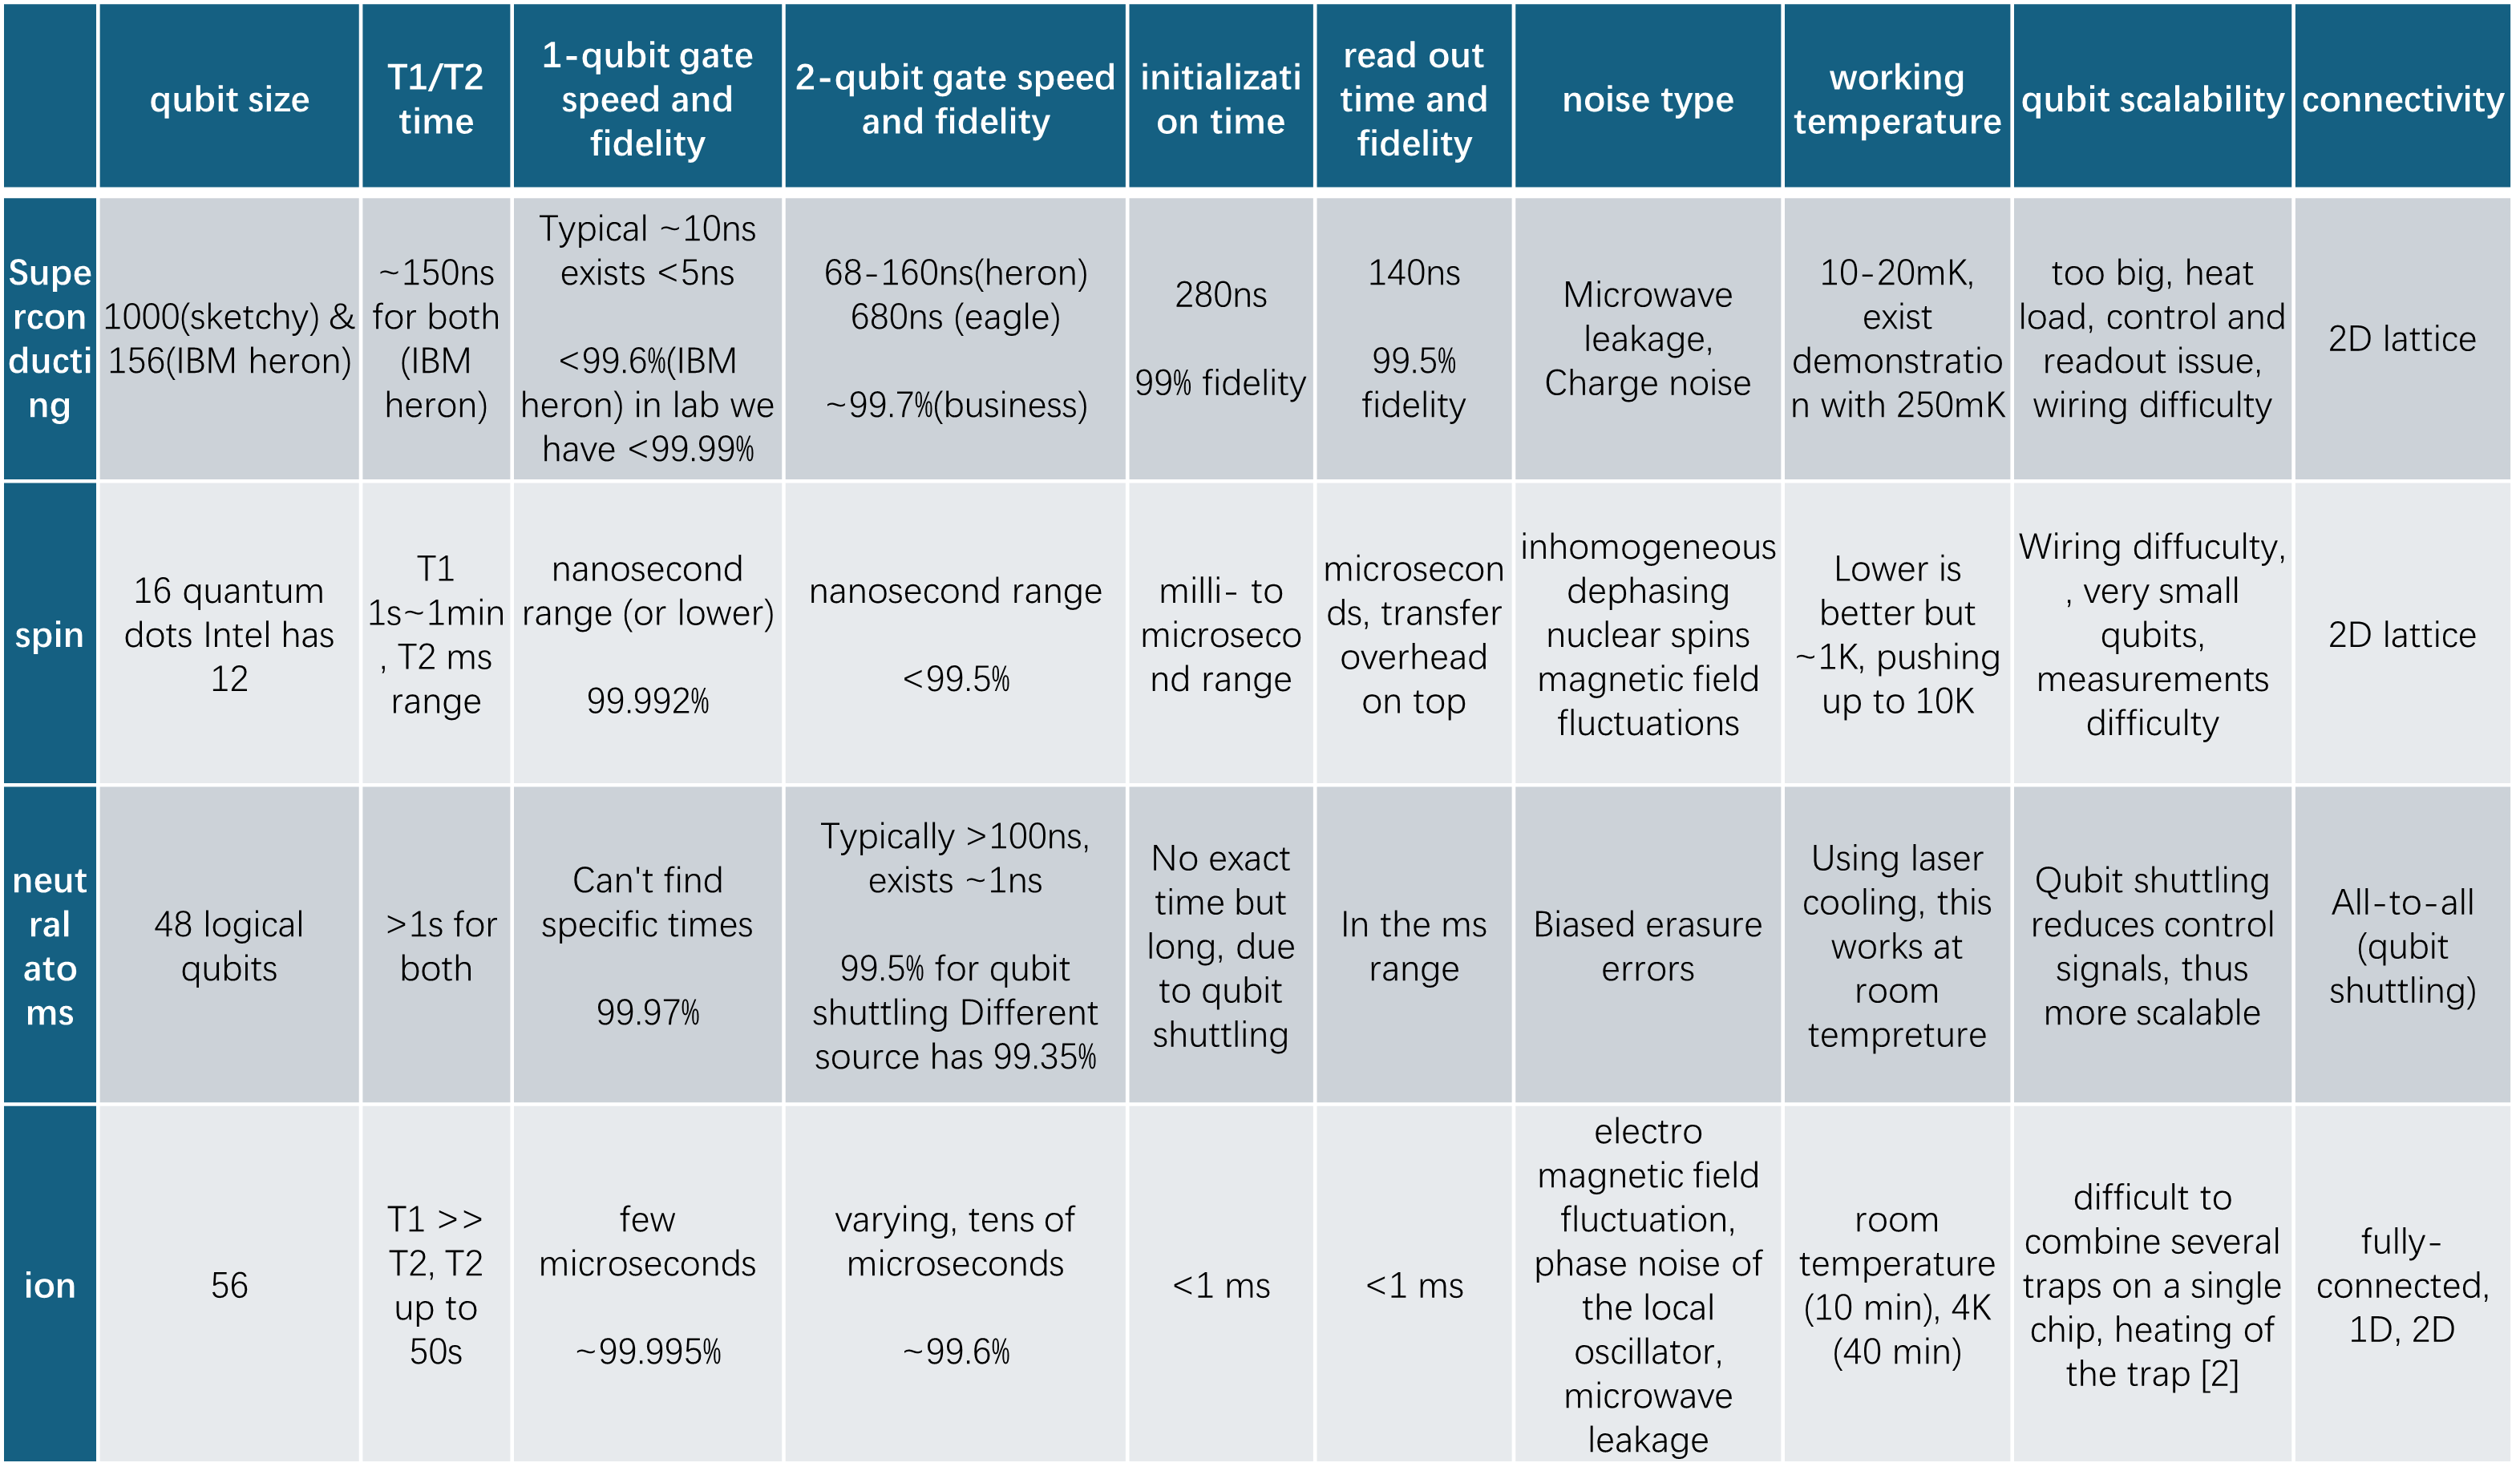
\includegraphics[width=1\linewidth]{images/compare.png}
    \caption{Comparison between different metrics for superconducting, spin, neutral atoms and ion qubits}
    \label{fig:enter-label}
\end{figure}
\end{comment}
% \begin{table}[ht]
% \small
% \centering
% \caption{Stuff}
% \label{tab:1}
%     \begin{tabular}{|p{1cm}|p{1.5cm}|p{1.5cm}|p{1.5cm}|p{1.5cm}|p{1.5cm}|p{1.5cm}|p{1.5cm}|p{1.5cm}|p{1.5cm}|l|} \hline  
%          \rowcolor[HTML]{2f7790}&  \textcolor{white}{Qubit Size}&  T1/T2 time&  1-qubit gate speed \& fidelity&  2-qubit gate speed \& fidelity&  initia-lization time&  readout time\& fidelity&  noise type&  working temperature&  qubit scalability&connectivity \\ \hline  
%          \rowcolor[HTML]{b6bac4} \cellcolor[HTML]{2f7790}super-conduc-ting&  j &  &  &  &  &  &  &  &  & \\ \hline  
%          \rowcolor[HTML]{d9dbe2} \cellcolor[HTML]{2f7790}spin&  &  &  &  &  &  &  &  &  &\\ \hline  
%          \rowcolor[HTML]{b6bac4} \cellcolor[HTML]{2f7790}neutral atom&  &  &  &  &  &  &  &  &  &\\ \hline  
%          \rowcolor[HTML]{d9dbe2} \cellcolor[HTML]{2f7790}ion&  &  &  &  &  &  &  &  &  &\\ \hline 
%     \end{tabular}
    
    
% \end{table}
%TC:ignore
\begin{table}[h]\begin{center}
    \caption{Comparison between different metrics for superconducting, spin, neutral atoms and trapped-ion qubits}
    \label{tab:qubit_comparison}
    \begin{tabular}{|>{\centering\arraybackslash}m{2cm}|>{\centering\arraybackslash}m{3.5cm}|>{\centering\arraybackslash}m{3.5cm}|>{\centering\arraybackslash}m{3.5cm}|>{\centering\arraybackslash}m{3.5cm}|}
         \rowcolor[HTML]{2f7790}&  \textcolor{white}{Superconducting Qubit}& \textcolor{white}{Semiconducting Qubit}&  \textcolor{white}{Neutral Atom Qubit}& \textcolor{white}{Trapped-ion Qubit}\\ \hline
         \rowcolor[HTML]{b6bac4} \cellcolor[HTML]{2f7790} \textcolor{white}{total qubits}&  1121 (IBM Condor)\cite{Afifi-Sabet_2023}, 156 (IBM Heron)\cite{IBMQuantum}& 16 \cite{Borsoi_2023} &  48 logical qubits, 280 physical qubits \cite{Bluvstein2024}& 56 \cite{quantinuum56} \\ \hline
         \rowcolor[HTML]{d9dbe2} \cellcolor[HTML]{2f7790} \textcolor{white}{T1/T2 time}&  $\sim$1.2 ms for both \cite{T1T2}& T1 1 min \cite{Camenzind_2018}, T2\textsuperscript{CPMG} 28 ms \cite{Veldhorst_2014} & T1$\gg$T2, T2 $\sim$40 s \cite{Barnes2022}& T1$\gg$T2, T2 up to 50 s \cite{wang2017single} \\ \hline
         \rowcolor[HTML]{b6bac4} \cellcolor[HTML]{2f7790} \textcolor{white}{1-qubit gate speed \& fidelity}& 4.16 ns\cite{Werninghaus_Egger_Roy_Machnes_Wilhelm_Filipp_2021}, $>$99.99\% \cite{T1T2}& ns range \cite{Stano_2022}, 99.992 \cite{Lawrie_2023}\% & $\mu$s range, 99.97\% \cite{Evered2023}& few $\mu$s, $\sim$99.995\% \cite{bruzewicz2019trapped} \\ \hline
         \rowcolor[HTML]{d9dbe2} \cellcolor[HTML]{2f7790} \textcolor{white}{2-qubit gate speed \& fidelity}& 68 ns (IBM Heron)\cite{IBMQuantum}, $\sim$99.9\%\cite{IQM} & 2 ns \cite{Malinowski_2019}, $\sim$99.81\% \cite{Mills_2022} & typically $>$100 ns \tablefootnote{\label{shuttling} This does not include shuttling time}, 99.5\% \cite{Evered2023}, exists 6.5 ns \cite{Chew2022}& varying, tens of $\mu$s, $\sim$99.6\% \cite{bruzewicz2019trapped} \\ \hline
         \rowcolor[HTML]{b6bac4} \cellcolor[HTML]{2f7790} \textcolor{white}{initialization time}& 180 ns, 99\% fidelity\cite{yoshioka2023activeinitializationexperimentsuperconducting} & ns range, $\sim$99.975\% fidelity \cite{Stano_2022} & $\mu$s to ms range, 99.8\% fidelity \cite{sunami2024scalablenetworkingneutralatomqubits}& $<$1 ms \cite{bruzewicz2019trapped}, 99.93\% fidelity\\ \hline
         \rowcolor[HTML]{d9dbe2} \cellcolor[HTML]{2f7790} \textcolor{white}{readout time}& 140 ns, 99.5\% fidelity\cite{Chen_2023} & $\mu$s range, $\sim$99.975\% fidelity \cite{Stano_2022}& 1 ms \cref{shuttling}, 99.8\% destructive \cite{Bluvstein2024}, 6 ms, 99.6\% non-destructive \cite{radnaev2024universalneutralatomquantumcomputer}& $<$200 $ \mu$s, 99.99\% fidelity \cite{myerson2008high}
or
$<$11 $\mu$s, 99.93\% fidelity \cite{crain2019high}\\ \hline
         \rowcolor[HTML]{b6bac4} \cellcolor[HTML]{2f7790} \textcolor{white}{noise type}&  leakage, charge noise, many others\cite{krantz_quantum_2019}& inhomogeneous dephasing, nuclear spins, magnetic field fluctuations \cite{Sun_2024} & biased erasure errors \cite{Sahay_2023}& EM field fluctuations, phase noise of local oscillator, microwave leakage \cite{wang2021single} \\ \hline
         \rowcolor[HTML]{d9dbe2} \cellcolor[HTML]{2f7790} \textcolor{white}{working temperature}&  250 mK\cite{anferov2024superconductingqubits20ghz} & $\sim$1 K, pushing towards 10 K \cite{Ono_2019} & laser cooling at vacuum room temperature \cite{Wintersperger2023}& room temperature (39 min), 4 K (90 min) \cite{wang2021single} \\ \hline
         \rowcolor[HTML]{b6bac4} \cellcolor[HTML]{2f7790} \textcolor{white}{connectivity}& 2D lattice\cite{IBMQuantum} & 2D lattice & fully connected, 2D, 3D \cite{Bluvstein2024}& fully connected, 1D, 2D \cite{valentini2024demonstration} \\ \hline
         \rowcolor[HTML]{d9dbe2} \cellcolor[HTML]{2f7790} \textcolor{white}{scalability}&  too big, heat load, control and readout wiring issue& wiring difficulty, small qubits, measurement difficulty& reduced control signals, $\gg 10^4$ atoms remains a challenge  \cite{sunami2024scalablenetworkingneutralatomqubits} & difficult to combine several traps on a single chip, heating of the trap \cite{large2024ion} \\ \hline
         
    \end{tabular}
    \end{center}
    
\end{table}
%TC:endignore
\subsection{Discrete Variable Quantum Systems}
These quantum system encode information in finite-dimensional Hilbert spaces, typically encoding information in two-level systems (qubits) or d-level systems (qudits).